\documentclass[10pt,article]{report}
\usepackage{amsmath}
\usepackage{graphicx}
\usepackage{booktabs}
\usepackage{array}
\usepackage[T1]{fontenc}
\usepackage{float}
\usepackage[utf8]{inputenc}
\usepackage{ctex}
\usepackage[utf8]{inputenc}
\usepackage{amsmath}
\usepackage{amssymb}
\usepackage{xcolor}
\usepackage{graphicx}
\usepackage{float}
\usepackage[utf8]{inputenc}
\usepackage[T1]{fontenc}
\usepackage{ctex}
\usepackage{amsmath}
\usepackage{amssymb}
\usepackage{xcolor}
\usepackage{graphicx}
\usepackage{float}
\usepackage{lmodern}
\usepackage{mathrsfs}
\usepackage{lipsum}
\usepackage{tikz}
\usepackage{braket}
\usepackage{adjustbox}
\usepackage{footmisc}
\usepackage{graphicx}
\usepackage{tcolorbox}
\setlength{\parindent}{0pt}
\title{数字电表}
\author{张世航}
\begin{document}
	\maketitle
	\section{200mV}
		\begin{table}[h]
			\centering
			\caption{200mV电压测量对比表}
			\label{tab:voltage}
			\begin{tabular}{l *{11}{c}}
				\toprule
				测量项 & \multicolumn{11}{c}{测量值 (mV)} \\
				\midrule
				$U_\text{改}$ & 0.001 & 20.05 & 40.05 & 60.19 & 80.05 & 100.02 & 120.15 & 140.13 & 160.11 & 180.14 & 199.64 \\
				$U_\text{标}$ & 0.00 & 20.0 & 39.9 & 60.0 & 79.9 & 99.8 & 119.9 & 139.8 & 159.8 & 179.8 & 199.2 \\
				$\Delta U$ & 0.001 & 0.05 & 0.15 & 0.19 & 0.15 & 0.22 & 0.25 & 0.33 & 0.31 & 0.34 & 0.44 \\
				\bottomrule
			\end{tabular}
		\end{table}
	\begin{figure}[H]
		\centering
		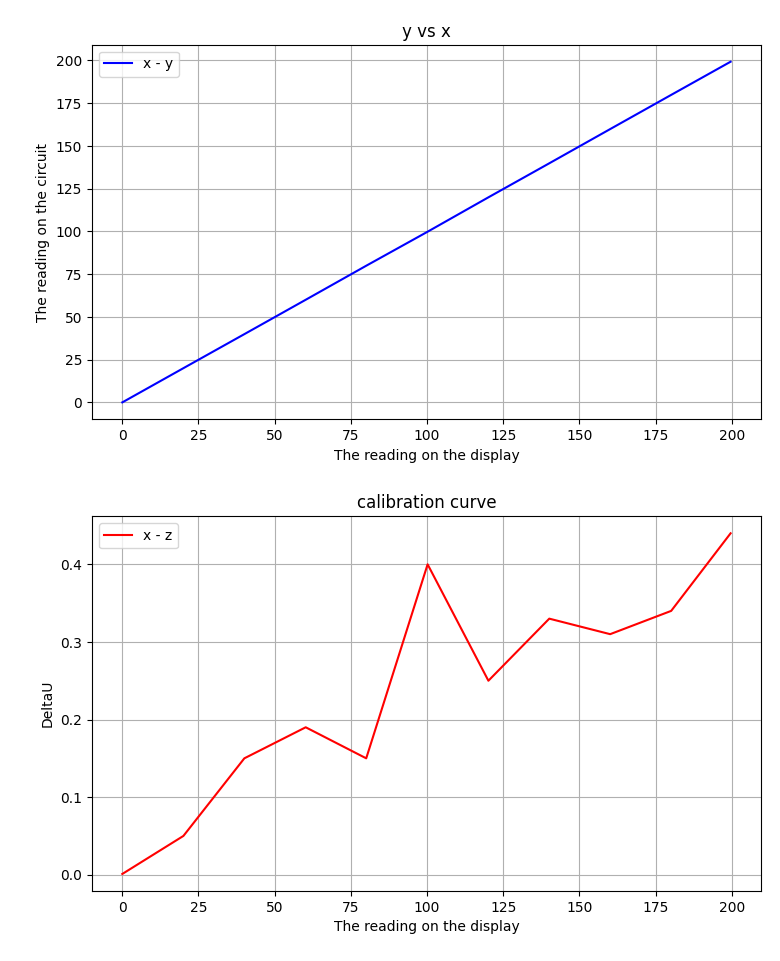
\includegraphics[width=0.7\linewidth]{200mV}
		\caption{200mV的示意图}
		\label{fig:figure1}
	\end{figure}
	
	
	\section{2V}
	\begin{table}[h]
		\centering
		\caption{2V电压测量对比表}
		\label{tab:voltage}
		\begin{tabular}{l *{11}{c}}
			\toprule
			测量项 & \multicolumn{11}{c}{测量值 (mV)} \\
			\midrule
			$U_\text{改}$ & 0.0001&0.2011&0.4020&0.6035&0.8037&1.0017&1.2015&1.4025&1.6037&1.8041&1.9942 \\
			$U_\text{标}$ &0.0000&0.2000&0.4000&0.6010&0.8010&0.9980&1.1980&1.3970&1.5970&1.7970&1.9870 \\
			$\Delta U$ & 0.0001 &0.0011& 0.002 & 0.0025& 0.0027& 0.0037& 0.0035 &0.0055& 0.0067& 0.0071&
			0.0072 \\
			\bottomrule
		\end{tabular}
	\end{table}
	\begin{figure}[H]
		\centering
		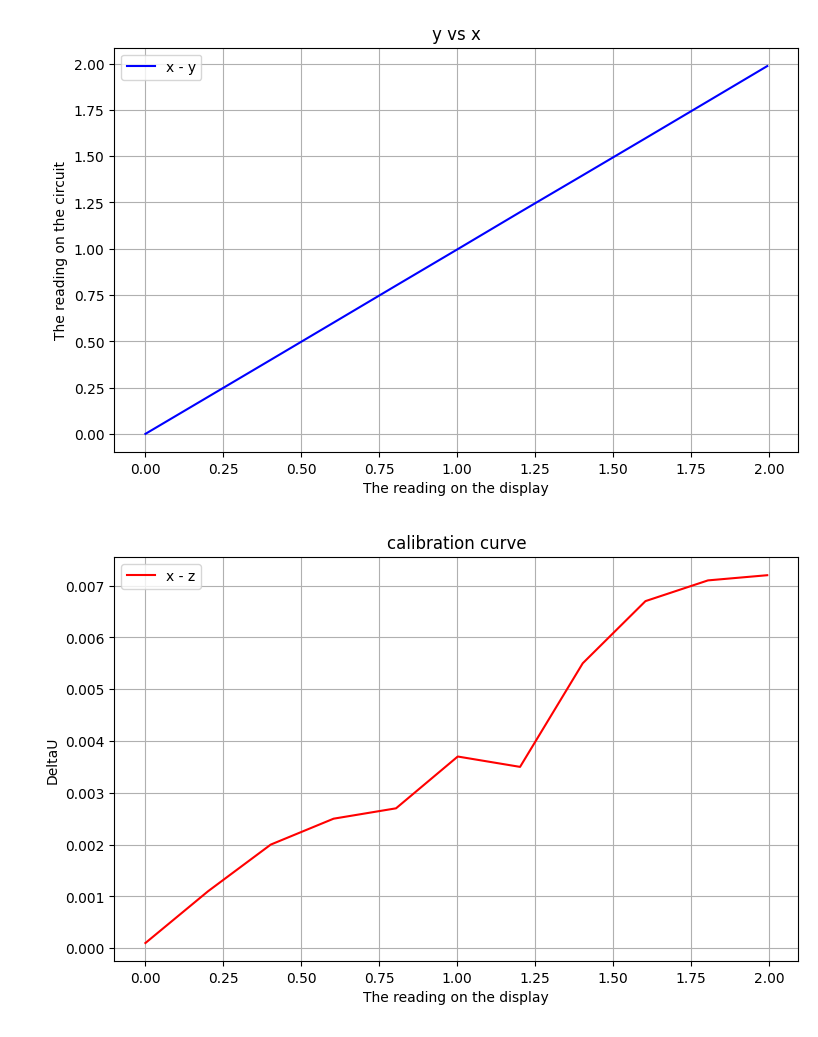
\includegraphics[width=0.7\linewidth]{2V}
		\caption{2V的示意图}
		\label{fig:figure2}
	\end{figure}

	\section{20mA}
	\begin{table}[h]
		\centering
		\caption{20mA电流测量对比表}
		\label{tab:voltage}
		\begin{tabular}{l *{11}{c}}
			\toprule
			测量项 & \multicolumn{11}{c}{测量值 (mV)} \\
			\midrule
			$I_\text{改}$ & 0.001&2.004&4.003&6.03&8.010&10.027&12.013&14.013&16.028&18.056&19.556\\
			$I_\text{标}$ &0.000&2.020&4.050&6.110&8.120&10.160&12.180&14.220&16.270&18.350&19.820 \\
			$\Delta I$ & 0.001 &-0.016& -0.047& -0.08 & -0.11&  -0.133& -0.167& -0.207 &-0.242 &-0.294&-0.264 \\
			\bottomrule
		\end{tabular}
	\end{table}
	\begin{figure}[H]
		\centering
		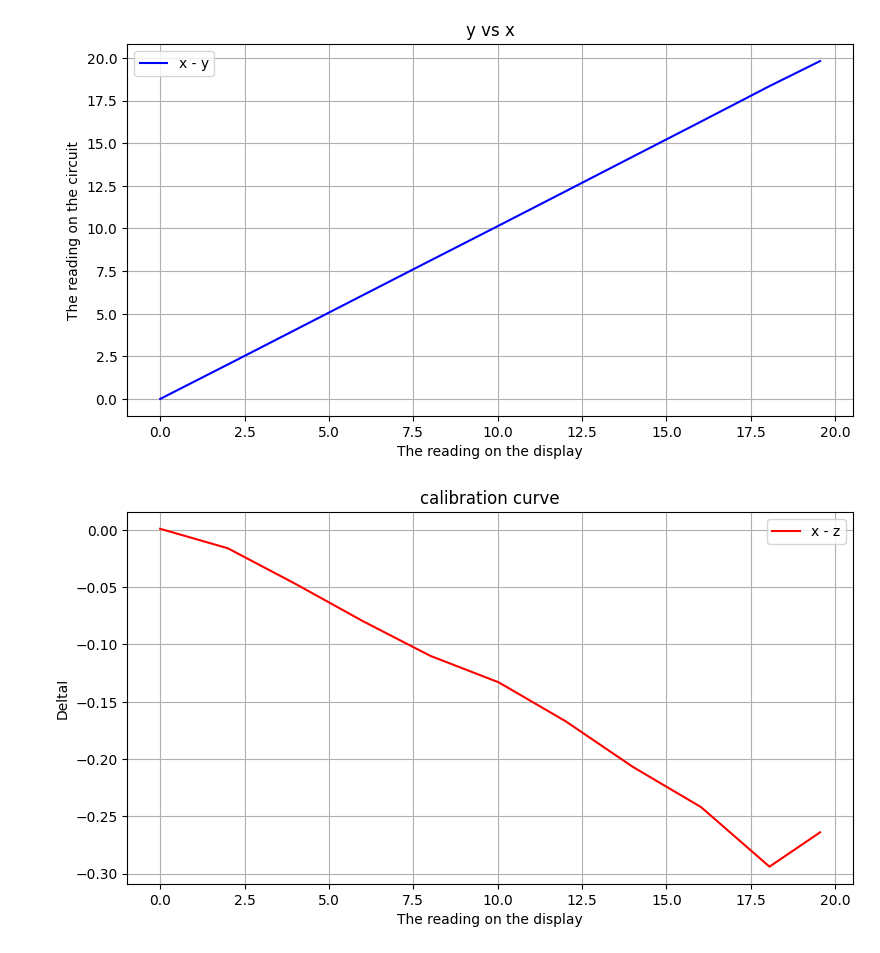
\includegraphics[width=0.7\linewidth]{20mA}
		\caption{20mA的示意图}
		\label{fig:figure3}
	\end{figure}
	
	
	\section{2mA}
	\begin{table}[h]
		\centering
		\caption{2mA电流测量对比表}
		\label{tab:voltage}
		\begin{tabular}{l *{11}{c}}
			\toprule
			测量项 & \multicolumn{11}{c}{测量值 (mV)} \\
			\midrule
			$I_\text{改}$ &0.000&0.204&0.402&0.609&0.803&1.004&1.202&1.402&1.604&1.802&1.999\\
			$I_\text{标}$ &0.000&0.200&0.390&0.600&0.800&1.000&1.200&1.400&1.600&1.800&1.990 \\
			$\Delta I$ & 0&0.004& 0.012& 0.009& 0.003& 0.004& 0.002& 0.002& 0.004& 0.002& 0.009 \\
			\bottomrule
		\end{tabular}
	\end{table}
	\begin{figure}[H]
		\centering
		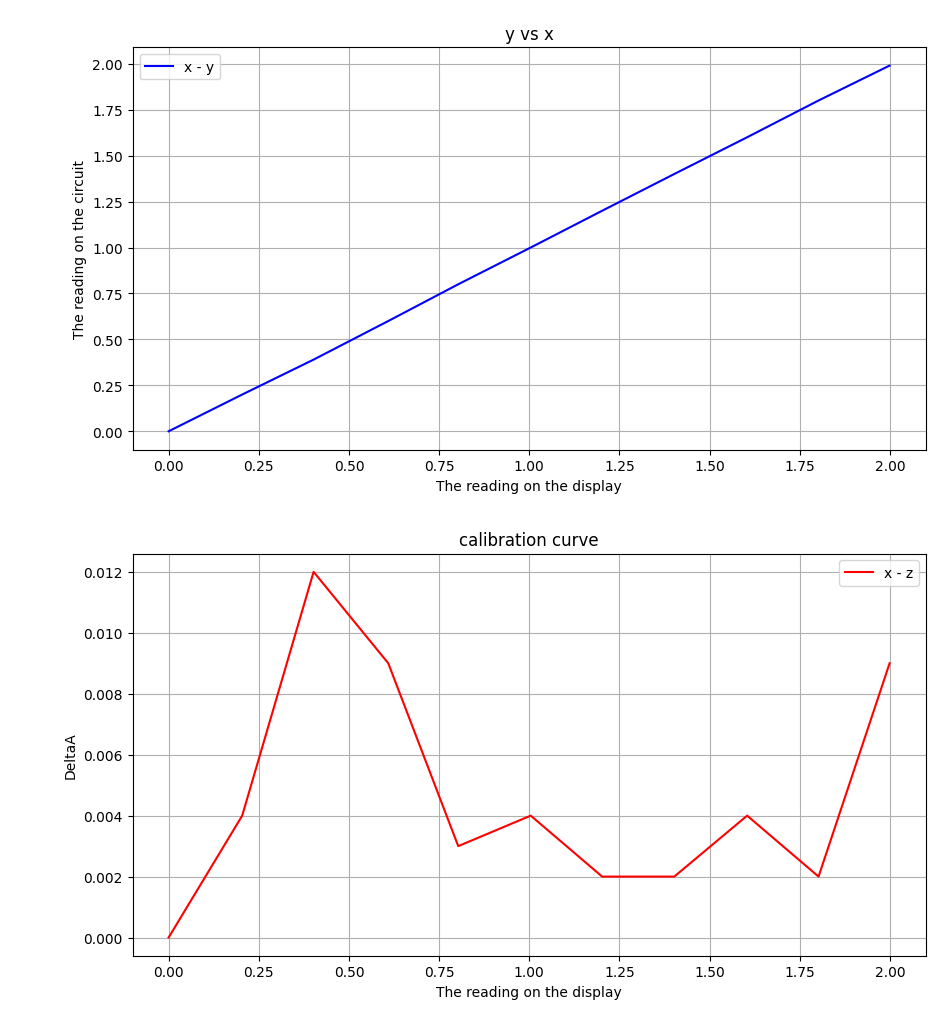
\includegraphics[width=0.7\linewidth]{2mA}
		\caption{2mA示意图}
		\label{fig:figure3}
	\end{figure}
	
\end{document}